\newpage
\subsection{Developing a Solution}
Creating something that tailors to the struggles of both designers and engineers requires a
carefully considered solution. Guided by a clear vision, an innovative idea, a solid system and a
flexible design language were developed.

\subsubsection{The Vision of High Quality Collaboration}
Before starting to think about solutions, the actual needs of the two parties have to be examined
and a clear vision needs to be set. To do this, the data of the survey done beforehand was used as a
foundation.

\begin{description}
      \item[The need for cross-disciplinary knowledge] - Both designers and developers would benefit
            from more knowledge about the other discipline at places where it matters most. If designers
            knew why using variables for design tokens or why applying Figma Auto-Layout in frames
            matters to devs, they could use these techniques more intentionally. Similarly, if
            developers knew how to use design tools to their advantage, they could skip tedious
            back-and-forth conversations and implement screens with more confidence.
      \item[The need for a shared understanding of components] - Designers should be aware that their
            structure of designs can, to a certain degree, mimic and influence the structure of
            code. As a component based approach is the golden standard of web development and found
            its way into interface design, both parties should share certain principles and best
            practices for components.
      \item[The need for more frequent communication] - Communication is key for frictionless
            collaboration and results in great products. As stated in the book Lean UX, the user experience
            is "created by a team, not an individual user interface designer".
            \directcite[63]{gothelfLeanUXProduktentwicklung2016} As remote working models become more
            popular, this becomes an even bigger challenge.
      \item[The need for common best practices] - Knowing when and why to use which tools and
            techniques would benefit the design handoffs drastically. Even more so, avoiding bad practices
            could save hours of reworking documentation, redoing designs or code implementations.
\end{description}

These four needs should be satisfied by the solution. The following sentence should serve as a
vision for the practical project.

% Something fancy incorporating all the needs specified above
\begin{figure}[H]
      \centering
      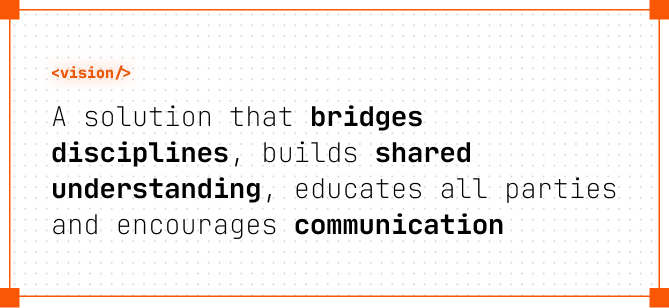
\includegraphics[width=300pt]{Chapter 5/Vision.png}
      \caption{Vision of hight quality collaboration (Source: own illustration)}
\end{figure}

\subsubsection{The Idea of a Shared Interface}
% Saying that the idea of an API is that no matter the platform there is a place that can be
% referred to, to get data, to be informed. Probably could take a page and quickly quote the
% definition of an API

% This concept can be applied to my practical work: A
% centralized place to get helpful tips, how-tos, best practices, communication ideas no matter the
% discipline. The DesignAPI is born: Design Alignment, Principles, Interchange. Being able to refer
% to it more often than once.

In programming realms, there is a widely known and used concept called API. Michael Goodwin
describes it perfectly saying an "API, or application programming interface, is a set of rules or
protocols that enables software applications to communicate with each other to exchange data,
features and functionality." \directcite{michaelgoodwinWhatAPIApplication2024} Upon hearing about a
great software, many devs respond with "Does it have an API?". This is because APIs are a place to
refer and get back to when you need functionality or data. It is a standard.

When it comes to the UI design process and the inter disciplinary collaboration, there is no such
thing as an API. Upon hearing about a great way to structure the design of components, no designer
would reply with "Is there an API for that?". My practical work aims to take the concept of an API
and create a centralized place to get helpful tips, how-tos, best practices and communication ideas
no matter the discipline.

The DesignAPI is born: Design Alignment, Principles, Interchange. It is a place designers as well as
developers can refer and get back to as soon as they need practical knowledge or a quick tip. It
serves as a standard of how design-dev collaboration should be done.

\subsubsection{The System Architecture}
% Explaining what the thing is actually made of: 
% 7 Categories, list each one and what it is about and opportunities for content to fit the needs as
% well: f.e. Figmafication: Opportunity to show devs why using Figma is beneficial.
% 
% For each category there is a set of cards and a set of so-called message templates
% - Consist of a front and a back. Front invites with a title and illustration, back a
%   selection of two to five sections that provide quick info. 

%
%   Explain each section: How to? - Why? - For Devs. Optional: Pro-Tip, Resource

% - Message Templates: To fit modern communication channels like Slack, MS Teams or others, there
%   are templates with Meme character. Again for each category at least one. Each one has a unique
%   purpose and aims to invite frequent playful communication with all team members. 

The DesignAPI starts with six selected categories. Each one covers a unique and challenging topic.

\begin{description}
      \item[States] - Focuses on component states like hover, focus or error that need to be
            designed before implementation. The opportunity for this category is to inform about
            existing states and how structuring them leads to less confusion on both design and
            development side.

      \item[Components] - Focuses on the definition of components, variants and their properties.
            The opportunity for this category is to get closer to a shared understanding of the
            concept of components between the disciplines.

      \item[Styleguide] - Focuses on fonts, colours, spacings or assets. The opportunity for this
            category is to outline the importance of well defined design tokens that can be shared
            between design and code.

      \item[Responsiveness] - Focuses on layouts across screen sizes. The opportunity for this
            category is to communicate best practices that make responsive design a shared
            principle.

      \item[Edge Cases] - Focuses on how general edge cases should be handled in design. The
            opportunity for this category is to reduce overall confusion about how the UI behaves in
            special cases.

      \item[Specials] - Focuses on remaining topics that deserve to be addressed. The opportunity of
            this category is to share little workflow tips for designers.
\end{description}

Each category has its own set of cards and so-called "Message Templates". They are designed to
address the specific opportunities within the category while trying to support the overall vision of
The DesignAPI.

\textbf{Cards}\\
% TODO DONE: write why I chose the card format
Inspired by "Laws of UX" by Jon Yablonski, The DesignAPI features cards that are designed for both
physical and digital use. There is something about this haptic format which makes rigid topics feel
fun and exciting. Like playing cards, the cards of The DesignAPI have a front and a back. The front
invites with a title and illustration and displays its category as well as the number of cards in
that category.
%%% TODO DONE: Add graphics that's like a blueprint of a card showing what's on every card (like my poster
%%% P-OWL)

\begin{figure}[H]
      \centering
      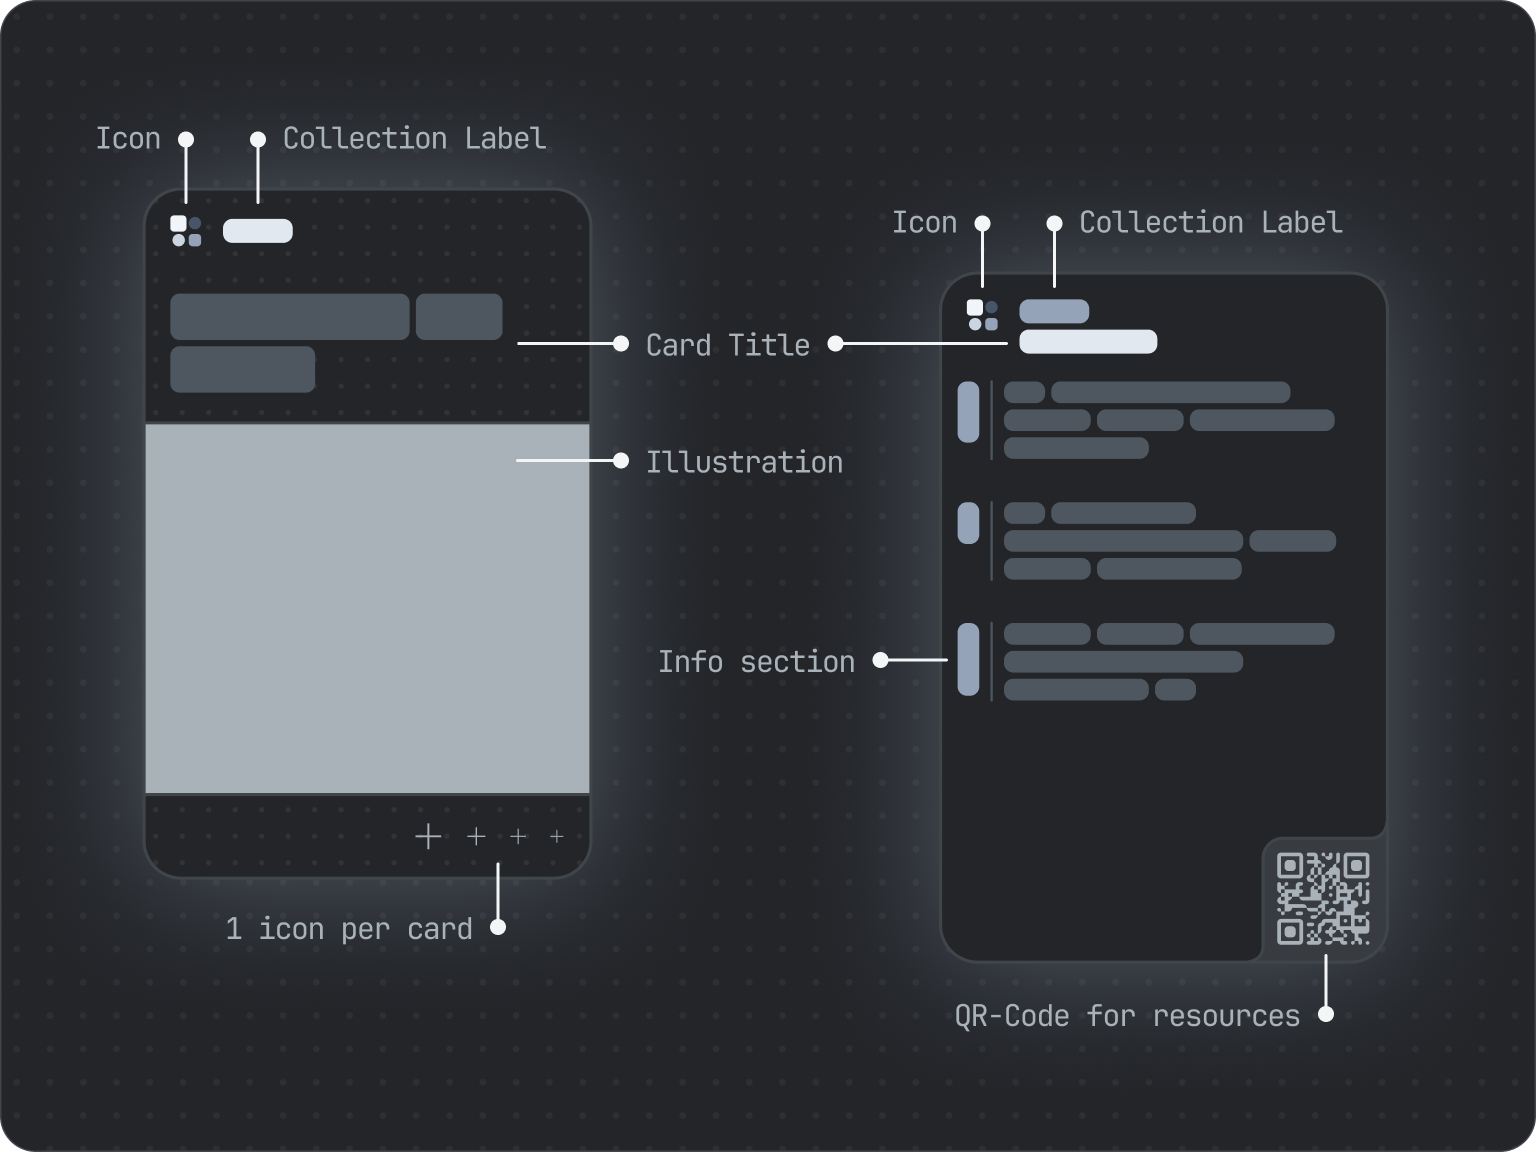
\includegraphics[width=300pt]{Chapter 5/Blueprint card.png}
      \caption{Blueprint of a card (Source: own illustration)}
\end{figure}

The back provides the user with information. It can have two to a maximum of five different sections
of content. Each section has its own purpose:

\begin{description}
      \item[How To?] - Explains what the basic idea or best practice is about and how to
            effectively use it in the everyday workflow.

      \item[Why?] - Outlines the background of the idea and why integrating it is beneficial for
            maximizing the quality of design.

      \item[For Devs] - For most topics, it is important for devs to know what it is about. This
            section brings them into the loop and also provides them with helpful tips. Also,
            designers can get a glimpse of their perspective.

      \item[Pro-Tip] - Often, there are opportunities for another tip on top of the "How To?"-section.
            This is the place for hands-on advice.

      \item[Resource] - Some ideas are communicated best with additional resources such as blog-posts,
            articles or videos. This section highlights that there is a QR-Code to scan to get to the
            external website.
\end{description}

\textbf{Message Templates}\\
% TODO DONE: write that these only make sense in a digital format Nah
The idea of Message Templates is to give team members a gentle nudge to share more design-related
messages with each other. Their purpose is not to replace existing communication, but to enhance it.
It should trigger a change in culture, so that a more frequent, open dialog between designers and
developers takes place.

To fit modern communication channels like Slack or MS Teams, the templates have a fun meme character
to them. This way every message is humorous, as well as informative and helpful.

In contrast to the cards, message templates do not have a rigid structure. As it is a template, they
are meant to be filled with individual content such as screenshots of UI, text or whatever is fits
the context of the template.

\subsubsection{The Design Language}
% Design language decisions
% Design has to be comfortable and inviting, so that users like picking it up and coming back to it often.

% Visual design colorful glass morphism: It should communicate transparency between the disciplines.
% It also adds depth (depth of information). A faint glow shows that it is somehow powerful and worth knowing
% The almost abstract illustrations keeps the content mysterious and interesting.
% (You want to look at the other side to see what it is about => invokes curiosity)

% Fonts and colours. Each category has its own colour shades. This makes it easy to distinct between
% the categories at a glance. 
% The selection of Fonts: 
% - Inter for paragraphs (great and versatile UI Font, default font in Figma
%   => makes designers feel right at home)
% - JetBrains Mono for headers (a font specifically made for developers)
% 
% Taken from both worlds of the spectrum, these fonts were the best choice for this project.

% TODO DONE: Chance for graphics showing different colours and stuff

% Voice and Tone:
% - To make the topic feel more casual all content is written in a rather informal way. 
The design of The DesignAPI must be well considered. It must be comfortable, inviting as well as
exciting, so that users like picking it up and get back to it once they need a tip.

\textbf{Visual Design}\\
% TODO DONE: Add graphics of this glassmorphism style
To meet these goals, The DesignAPI adopts a colourful glass morphism style. The glass-like elements
communicate transparency between disciplines, while layering the elements gives the design depth
much like the richness of information conveyed on the cards.

All unique illustrations are kept in a minimalistic, almost abstract style that makes the viewer
interested in what it is actually about. A faint glow shows that the information is powerful and
worth knowing.

\begin{figure}[H]
      \centering
      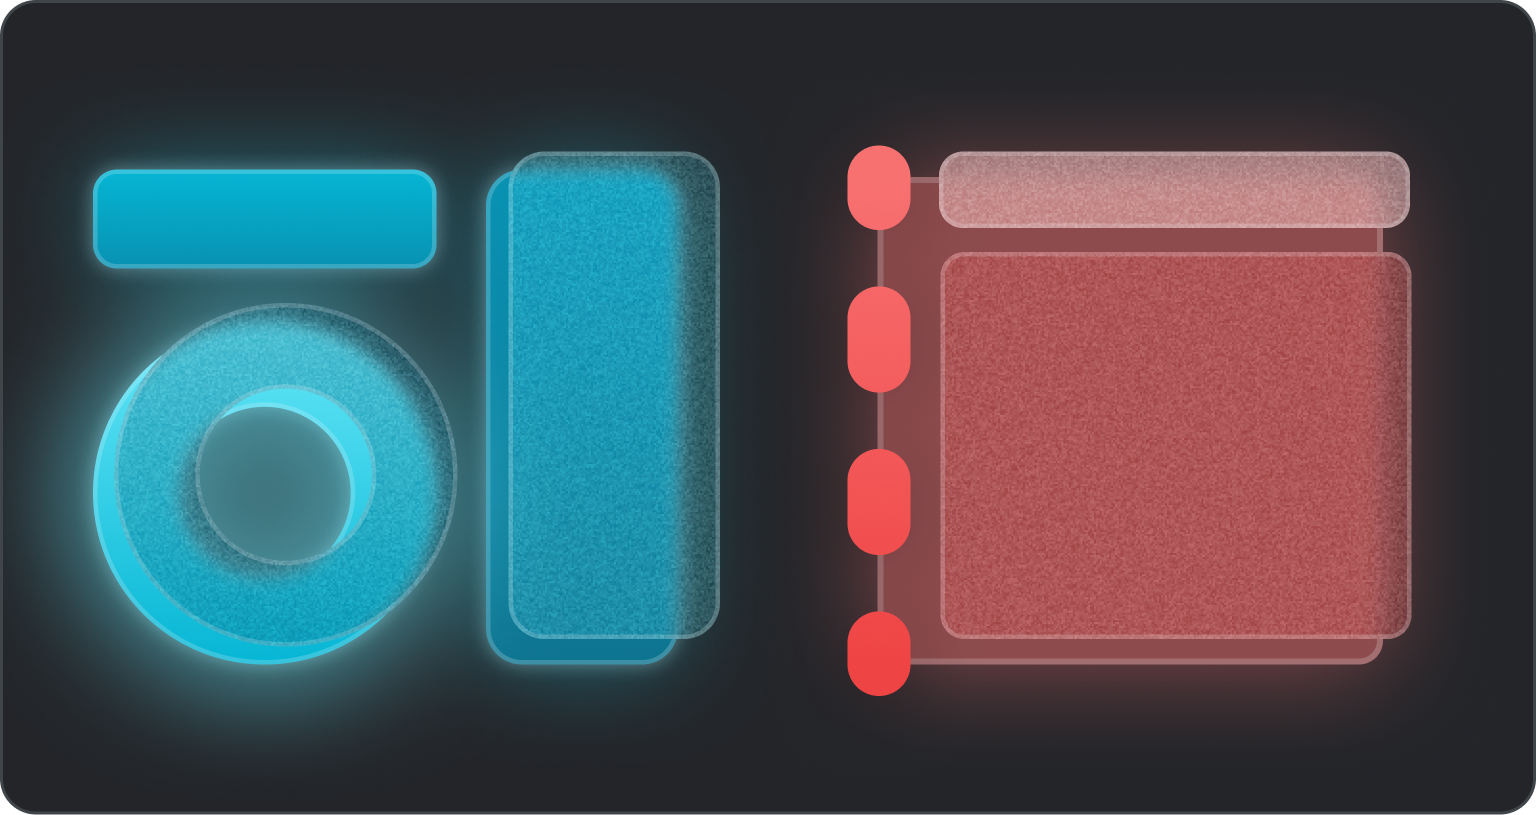
\includegraphics[width=300pt]{Chapter 5/glassmorphism style.png}
      \caption{Visual design: Glass Morphism (Source: own illustration)}
\end{figure}

\textbf{Fonts, Iconography and Colours}\\
Each category has its own primary colour and a number of shades that can be used for icons and
illustrative elements. Furthermore, an individual icon was designed for each category to be able to
easily distinct between them without solely relying on colour.

Moreover, a dark and light mode for all assets using semantic design tokens was integrated, to
make it even more appealing for the target group and to allow for a bit of personalization.
% TODO DONE: Add graphics for colours and category icons

To show the dual nature of The DesignAPI's target audience, the following two typefaces were chosen:
\begin{description}
      \item[Inter] - Used for paragraphs. It is a massively popular typeface mostly used in
            computer interfaces and is the default font in Figma. Using this font, contributes to a
            sense of familiarity for UI designers. \vglcite[]{rasmusanderssonInterTypefaceFamily}

      \item[JetBrains Mono] - Used for headings. It is a typeface made for developers to increase
            readability in code editors. With this font, the goal was to make developers comfortable
            using The DesignAPI. \vglcite[]{jetbrainss.r.o.JetBrainsMonoTypeface}

      \item[Gochi Hand] - Used for author notes. It is an informal font that should resemble a normal
            persons handwriting. This font was used to add useful notes on top of the cards rigid structure
            to add important information and make them feel more lively. \vglcite[]{huertatipograficaGochiHand2020}
\end{description}

\begin{figure}[H]
      \centering
      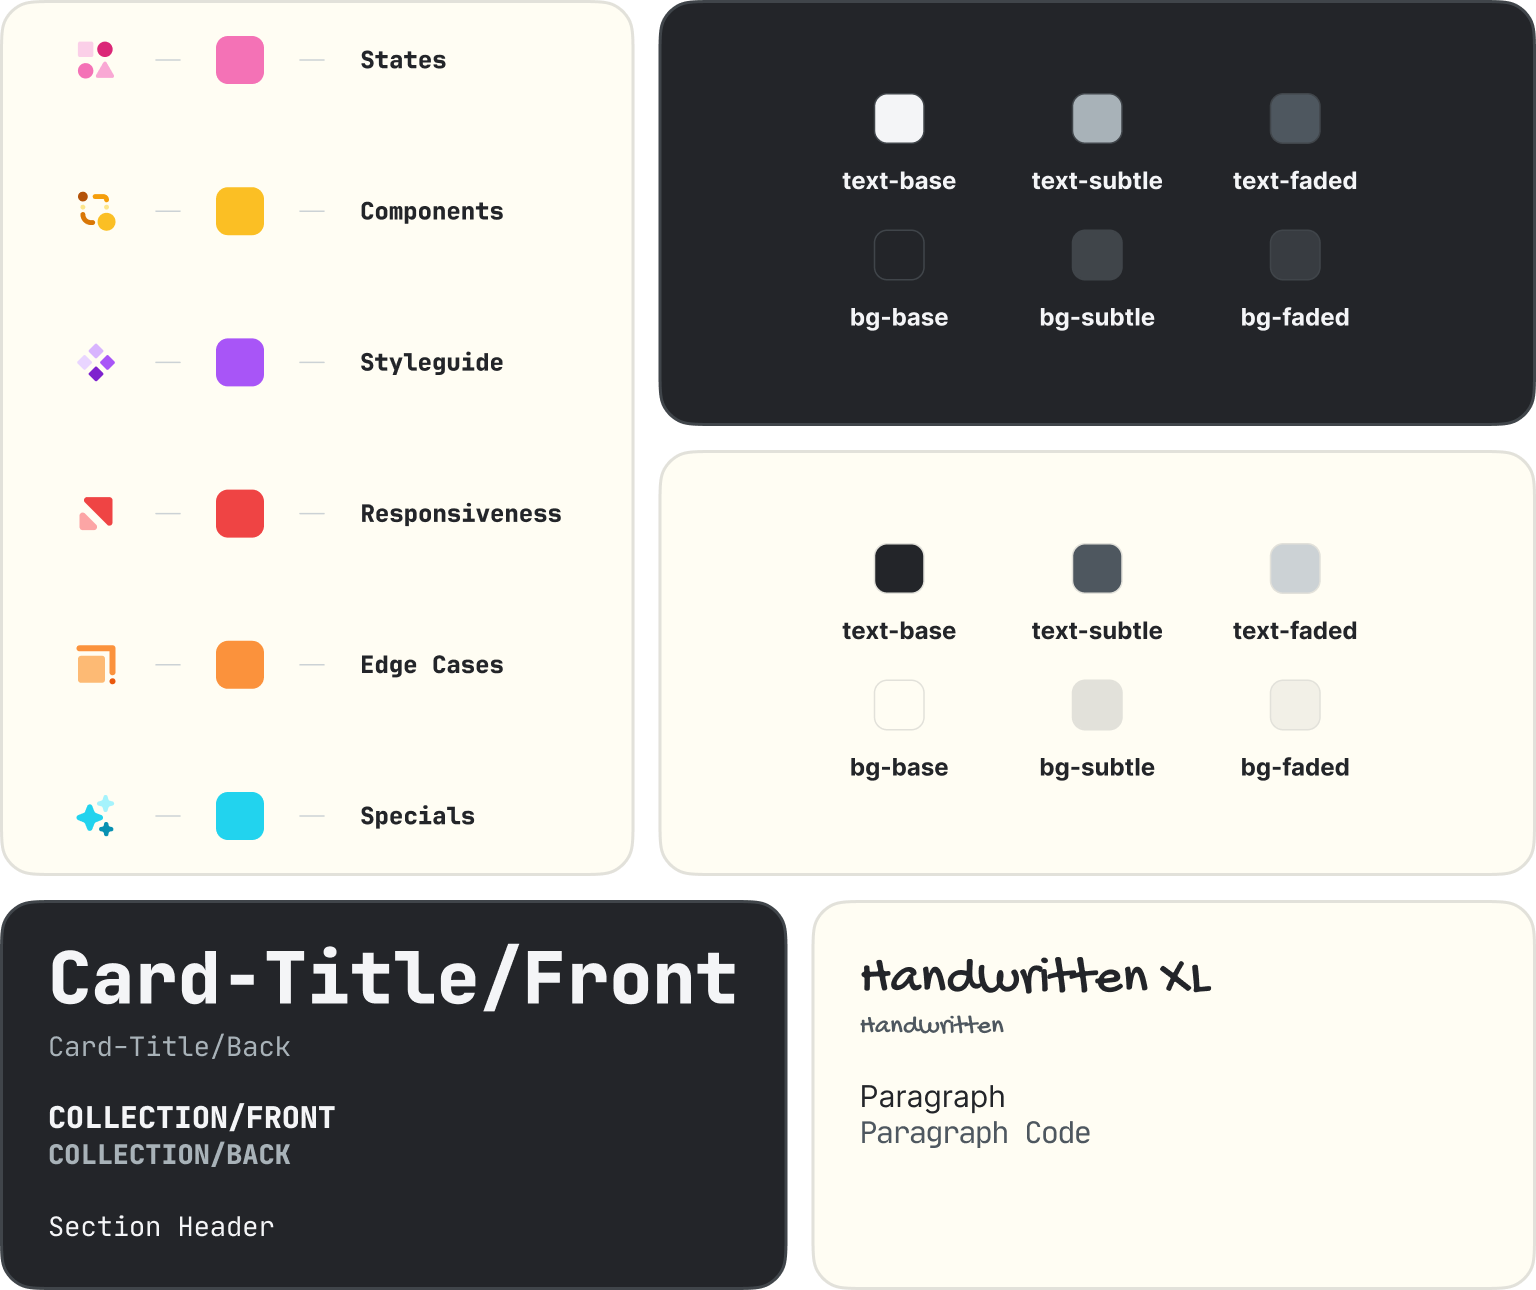
\includegraphics[width=300pt]{Chapter 5/Icons Colors Fonts.png}
      \caption{Fonts, Iconography and Colours (Source: own illustration)}
\end{figure}

% TODO DONE: Add graphics for the fonts in a nice presentation. Maybe all Figma styles

\textbf{Voice and Tone}\\
Reading best practices and guidelines can be exhausting quickly, as their formulation is often very
technical and rigid. The DesignAPI took inspiration from a study examining how different tones of
voice affects the impressions of desirability, trustworthiness and friendliness for a brand.
The study states that "dry industries [...] can benefit from a little conversational language".
\directcite{katemoranImpactToneVoice2024}

Additionally, casual and somewhat enthusiastic language generally performs best as it keeps
desirability and trustworthiness high. \vglcite{katemoranImpactToneVoice2024}
The following figure shows examples of the language used in The DesignAPI.

\begin{figure}[H]
      \centering
      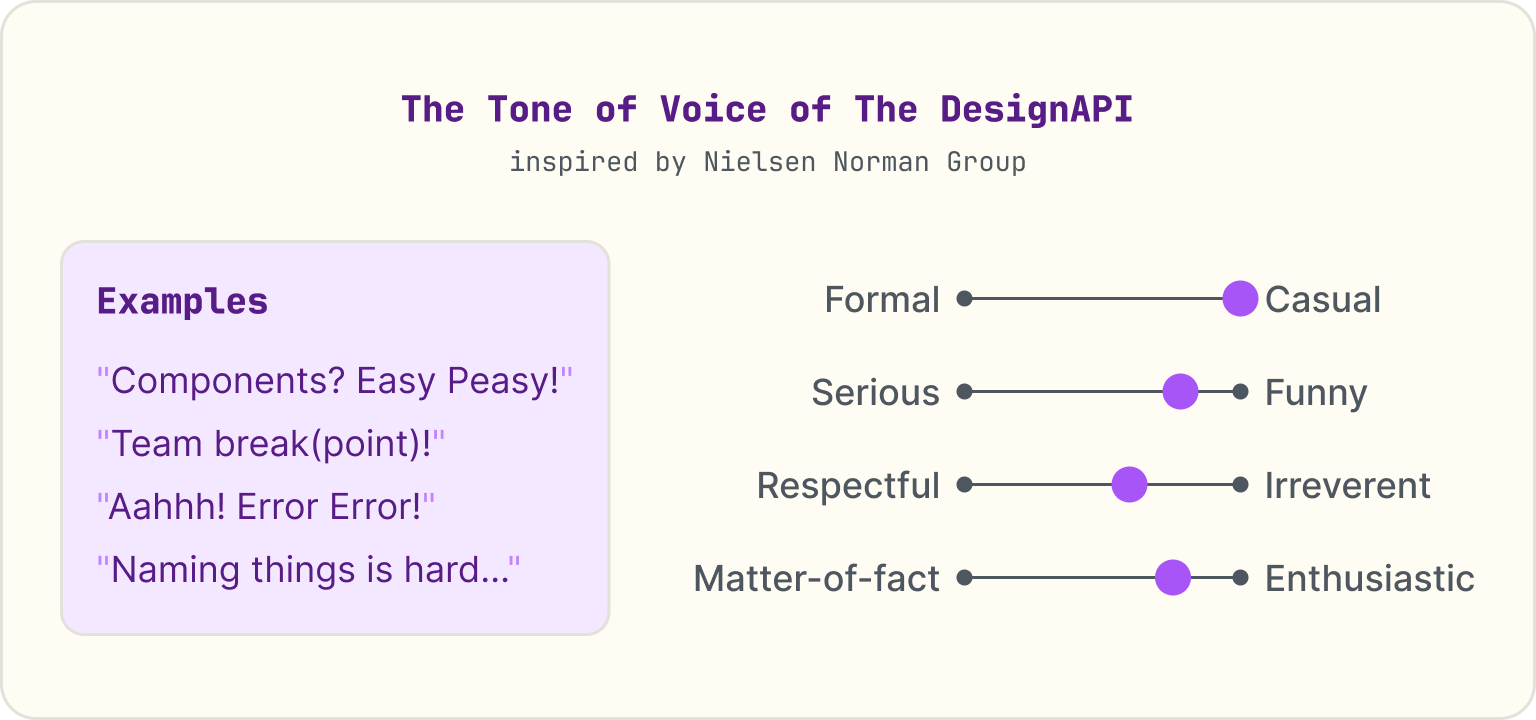
\includegraphics[width=300pt]{Chapter 5/Voice of Tone.png}
      \caption{Voice of Tone (Source: own illustration based on Nielsen Norman Group https://www.nngroup.com/articles/tone-voice-users/)}
\end{figure}
% TODO DONE: Add graphics with these examples and include a graph like this:
% https://media.nngroup.com/media/editor/2024/01/30/example-3.jpg
